\section{Results \& Evaluations}
In this chapter, we perform evaluation on our model and the other algorithms. 
%The repository of our model is provided in github \footnote{\url{https://github.com/cwleung/LKJTM}}.
\subsection{Experiment Testing}
The experiment will be conducted with a number of existing proposed topic models as mentioned related work section above. We conduct the experiment with those baseline algorithms and evaluate them in terms of accuracy and running time. Some of the source code of competitive were provided by their authors in Github\footnote{For instance, Correlated Topic Model(CTM), \href{https://github.com/blei-lab/ctm-c}{https://github.com/blei-lab/ctm-c}}. The outcome result will be extensively studied and conclude the insight behind the algorithms and methodologies. Detail to be stated in section \ref{ch4:result_model}. Our probabilistic part of model implemented using Pyro\cite{bingham_pyro_2019}, while the model optimization and transformer implementations are based on PyTorch\cite{paszke_automatic_2017}.
\subsection{Dataset}To evaluate the performance of the model, we selected \textit{20Newsgroups} and \textit{Reuters-21578} data sets in our evaluation stage. 20Newsgroups consist of 18,846 news group documents \footnote{\url{http://qwone.com/~jason/20Newsgroups/}} and the Reuters-21578 includes 10,788 documents in total. Both of the dataset will be preprocessed to remove stop-words and stemming before the evaluation. Both data set were separated into training/testing set for training and evaluation process.
% 20newsgroups
\textit{20Newsgroups} data set contains around 20,000 newsgroups documents, which divided into 20 different groups. In the preprocessing stage, we remove the document with only one word. We filter the stop-words, remove the word with special characters. The frequency of words are limited to between 2\%-50\%. After the preprocessing, the data set was split into 11314, 7532 documents with 5651 vocabularies. 
% reuter 21578
\textit{Reuter-21578} data set is a collection of documents from Reuters newswire in 1987. After performing the preprocessing, the processed data set consist of 7769, 3019 documents for train/test documents with 1622 vocabularies.
% preprocessing
On the data preprocessing stage, we perform tokenization, stopword removal, lemmatization on the documents.
\subsection{Models}\label{ch4:result_model}
We compare the model performance with a numbers of rivals. We take Latent Dirichlet Allocation (LDA)\cite{blei_latent_2003} as the baseline model. Other models include Transformer\cite{vaswani_attention_nodate}\footnote{Not a topic model, but we think it is worth to make comparison still.},  ProdLDA\cite{srivastava_autoencoding_2017} and Embedded Topic Model(ETM)\cite{dieng_topic_2019}.
% LDA
LDA fits the model with with mean-field variational inference \footnote{Adopted from \textmd{scikit-learn} library}
% ProdLDA
ProdLDA, a topic model learning using amortized inference to approximate the variational distribution on document-topic proportion.
% ETM
ETM model, a topic model built on top of ProdLDA model, uses dot-product of word embedding and topic embedding to represent the topic-word distribution $ \beta $.
\subsection{Algorithmic Settings}
% optimization algorithm
To perform posterior inference, we employed Stochastic Variational Inference (SVI) \cite{hoffman_stochastic_2013} for the optimization problem. We set the minibatch size to 512 documents.
% Other model
For LDA, we applied the model provided from sklearn package (version 0.24.0) \footnote{Sklearn website \url{https://scikit-learn.org/stable/index.html}}. For ETM, we run the experiment with the parameter suggested \cite{dieng_topic_2019}. For ProdLDA, we perform optimization with inference network architecture as described in the paper \cite{srivastava_autoencoding_2017}. 
% epochs
To train the models, every model run on 200 epochs to give the best performance. 
% learning rate
To perform optimization, we use Adam for the gradient ascent algorithm, and we set the learning rate to 2e-3.
% l2-regularization factor
we use $ l2 $-regularization to the 1e-5,
% inference network [size, activation function, dropout, batch-norm]
We applied the settings from \cite{srivastava_autoencoding_2017} to perform amortized inference. The inference architecture included 300 dimension of hidden layers. 
% embedding dimension 512
The dimension for embedding $ \rho $ are set to 256.
% Transformer settings
For the Transformer model settings, we define the sequence length to 20, number of head to 8, and 4 layer stacks of transformer encoder and 256 hidden dimension.
\subsection{Quantitative Result}
Perplexity has been known for evaluating the fitness of NLP models, however it may not be the best metrics to examine the wellness of a topic model\cite{newman_automatic_nodate}.
Secondly, in order to compute the perplexity for topic model using AEVB, we follow the previous work, using the variational lower bound to compute the perplexity.
For the same reason, the perplexity may not perfectly reflects the true quality of a topic model. 
Hence, we take the topic coherence \cite{mimno_optimizing_2011} as the main measure to evaluate the models.
Also, sometimes even a topic model could obtain a high coherence score, the topics could be repeated many times that yields poor result. 
We also implemented topic diversity \cite{dieng_topic_2019} as one of the measure of topic model, the measure that evaluate how well each topic contains distinct word from other topics. 
In this section, we evaluate the model with the following metric : Perplexity, Topic Coherence (TC), Topic Diversity (TD).
\begin{table}[h]
\centering
\begin{tabular}{lllllll}
\hline
\#Topic     & \multicolumn{3}{c}{k=20} & \multicolumn{3}{c}{k=50} \\
Metrics     & PPL     & TC     & TD    & PPL     & TC     & TD    \\ \hline
LDA     & 478.8 & \textbf{0.248} & 0.702 & 507.1 & 0.193 & 0.554 \\
ETM     & 279.0 & 0.213 & 0.500 & 336.8 & 0.200 & 0.211 \\
ProdLDA & 796.6 & 0.188 & \textbf{0.792} & 521.8 & 0.180 & \textbf{0.609} \\
TECTM   & \textbf{259.6} & 0.237 & 0.586 & \textbf{263.0} & \textbf{0.226} & 0.367
\\ \hline
\end{tabular}
\captionof{table}{Result for Reuters-21578 dataset\label{tbl:result2}}
\end{table}
\begin{table}[h]
\centering
\begin{tabular}{lllllll}
\hline
\#Topic     & \multicolumn{3}{c}{k=20} & \multicolumn{3}{c}{k=50} \\
Metrics     & PPL      & TC      & TD  & PPL      & TC      & TD  \\
\hline
LDA     & 2442.7 & 0.168 & \textbf{0.774} & 2538.2 & 0.154 & \textbf{0.713} \\
ETM     & \textbf{1640.5} & 0.191 & 0.592 & \textbf{1715.5} & 0.159 & 0.337 \\
ProdLDA & 6018.5 & 0.072 & 0.734 & 9057.9 & 0.014 & 0.703 \\
TECTM   & 1954.4 & \textbf{0.200} & 0.630 & 1944.6 & \textbf{0.194} & 0.509 \\
\hline
\end{tabular}
\captionof{table}{Result for 20Newsgroups dataset\label{tbl:result1}}
\end{table}
\paragraph{Reuters-21578}
% Reuter-21578
On the data set Reuter-21578, our model perform the best in perplexity, with 259.6 and 263.0 when k=20 and k=50 respectively. Our model also performs the best on topic coherence when $ k=50 $, where it is 0.226, with a competitive topic coherence score when $ k=20 $ as well. To focus on TD score, our model did not beat the best model, but also maintain a good enough TD score to generate variety of topics, with $ 0.586 $ and $ 0.367 $ when $ k=20 $ and $ k=50 $ respectively.
% our model 
% discussion
As result apparently our model perform well on several metrics. 
\paragraph{20Newsgroups}
% best model
On the result from table \ref{tbl:result1}, displays that our model has outperform the other model by TC score. On perplexity score, ETM obtain the best score when $ k=20 $ and $ k=50 $. On the other hand, LDA has the best TD score on both $ k=20 $ and $ k=50 $. It can 
% our model
When $ k=20 $, our model has 1954.4 in perplexity score, 0.200 TC score and 0.630 in TD score. When $ k=50 $, our model has 1944.6 in perplexity score, 0.194 TC score and 0.509 in TD score.
ProdLDA, perform the worse in both perplexity and topic coherence score.
% discussion
\paragraph{}It can be seen that, when the number of topic increases, the topic model performance decrease proportionally.
For instance, ProdLDA has a quite well metric score on small data set such as Reuters-21578. However, it performance drag down drastically on a bigger data set such as 20Newsgroups.
Also we observe that when our model is capable to maintain a relatively good topic coherence score when the topic increase from the result above.
% TODO comparison to LDA
To compare with LDA, it could obtain a high enough TC and TD scores in our experiment settings, however our model does better in TC scores in both topic numbers we conducted investigations.
\subsection{Training}
From figure \ref{fig:ppl20t}, \ref{fig:ppl50t}, display the training process of the training loss and log probability by 200 epochs. We observe that the negative log probability is decreasing over epochs. For the metrics, the topic coherence and the topic diversity improves slowly along the training proceeds, the perplexity also decreases along.
\subsection{Qualitative Result}The proposed model will be evaluated with a number of specifically selected topic and examined with their performance separately. The result will be exhaustively compared with other existing models.\\
From table \ref{tbl:t3}, we have selected some topic words each model generated from 20Newsgroups when $ k=20 $. The topics represent space, operating system, religion, encryption and guns respectively. Our model has shown capability on capturing key words from each topic, such as on topic "space": \textit{nasa}, \textit{space}, \textit{jpl}, \textit{moon}, \textit{earth}, \textit{station}, \textit{flight} are the outputs.
\begin{table}[ht]
\centering
%\scriptsize
\begin{tabular}{llll}
\hline
Our Model  \\ \hline
\textbf{nasa }gov \textbf{space jpl moon earth station flight }research digex\\
\textbf{windows window }problem \textbf{dos }running \textbf{file mouse }mit de ms\\
\textbf{god jesus christian }people faith bible time church good things\\
\textbf{key }chip \textbf{encryption }clipper \textbf{security }\textbf{privacy }government \textbf{keys }public escrow\\
\textbf{gun }people control government \textbf{guns weapons }american make clinton state \\ \hline
\hline
ProdLDA  \\ \hline
\textbf{nasa} \textbf{space} gov people \textbf{station} \textbf{time} \textbf{orbit} dc program shuttle \\
\textbf{scsi} \textbf{drive} \textbf{controller} max \textbf{drives} \textbf{ide} senior \textbf{tape} time people \\
\textbf{god jesus atheists christian bible religion atheism christians} word truth \\
\textbf{key crypto} session nt chips chip \textbf{serial} dos \textbf{keys} \textbf{encrypted} \\
\textbf{gun }people god religion writes life morality ohio argument question \\ \hline
\hline
LDA  \\ \hline
\textbf{space, nasa}, gov, access, \textbf{launch, earth}, digex, \textbf{moon, orbit}\\
\textbf{file, window, program, ftp}, \textbf{files}, \textbf{server}, \textbf{image, graphics, windows}\\
\textbf{god}, people, \textbf{jesus}, \textbf{christian}, \textbf{bible}, writes, life, \textbf{christians}, time\\
\textbf{key}, \textbf{encryption}, chip, clipper, \textbf{keys}, \textbf{security}, \textbf{government}, \textbf{privacy}\\
\textbf{gun, guns, law, police}, people, \textbf{weapons, crime, fbi}, control
\\ \hline
\hline
ETM  \\ \hline
\textbf{space, nasa}, gov, mr, president, health, research, year, center\\
\textbf{windows, file, window, program, files, server}, \textbf{version}, dos, \textbf{image}\\
\textbf{god}, people, \textbf{jesus}, \textbf{christian}, \textbf{israel}, \textbf{bible}, \textbf{jews}, \textbf{christians}, \textbf{israeli}\\
\textbf{key, encryption}, chip, clipper, \textbf{keys}, \textbf{privacy}, \textbf{security}, technology, government\\
\textbf{gun}, people, government, \textbf{law}, state, \textbf{guns}, article, \textbf{weapons}, control
\\ \hline
\end{tabular}
\captionof{table}{Top-9 words for each topic from 5 topics selected\label{tbl:t3}}
\end{table}
\begin{figure}
\centering
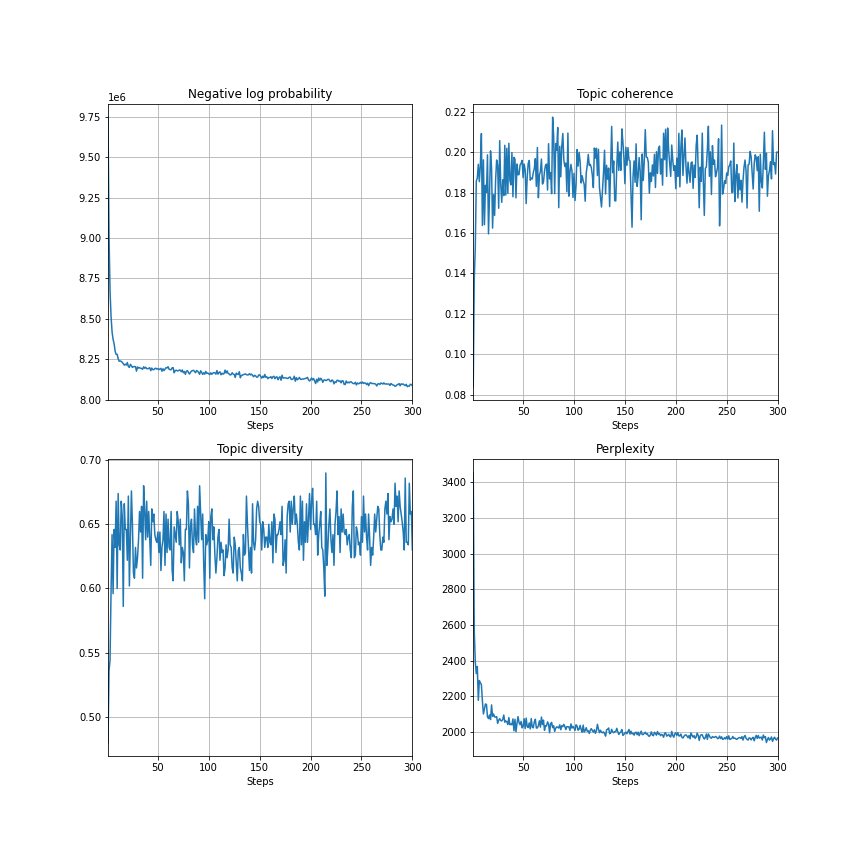
\includegraphics[width=1\linewidth]{figures/0106/ppl_20t}
\caption{20Newsgroups (k=20)}
\label{fig:ppl20t}
\end{figure}
\begin{figure}
\centering
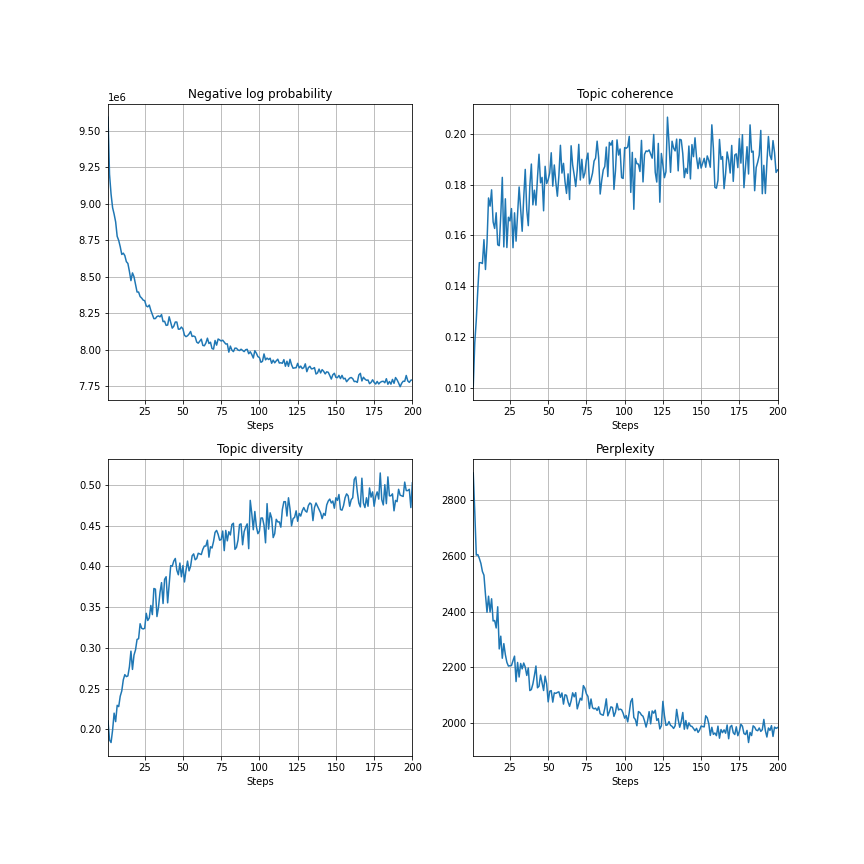
\includegraphics[width=1\linewidth]{figures/0106/ppl_50t}
\caption{20Newsgroups (k=50)}
\label{fig:ppl50t}
\end{figure}
%\begin{figure}
%\centering
%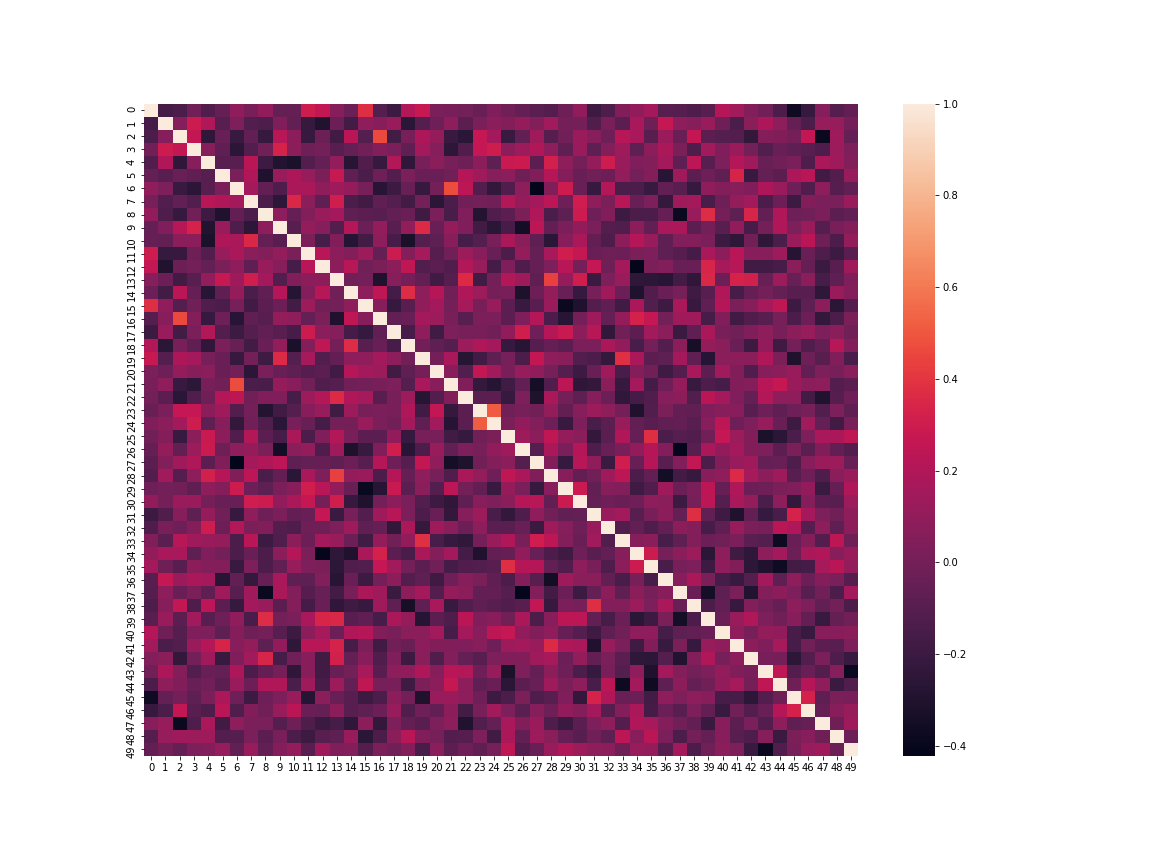
\includegraphics[width=0.7\linewidth]{figures/0106/hm_50t}
%\caption{}
%\label{fig:hm50t}
%\end{figure}
%\begin{figure}
%\centering
%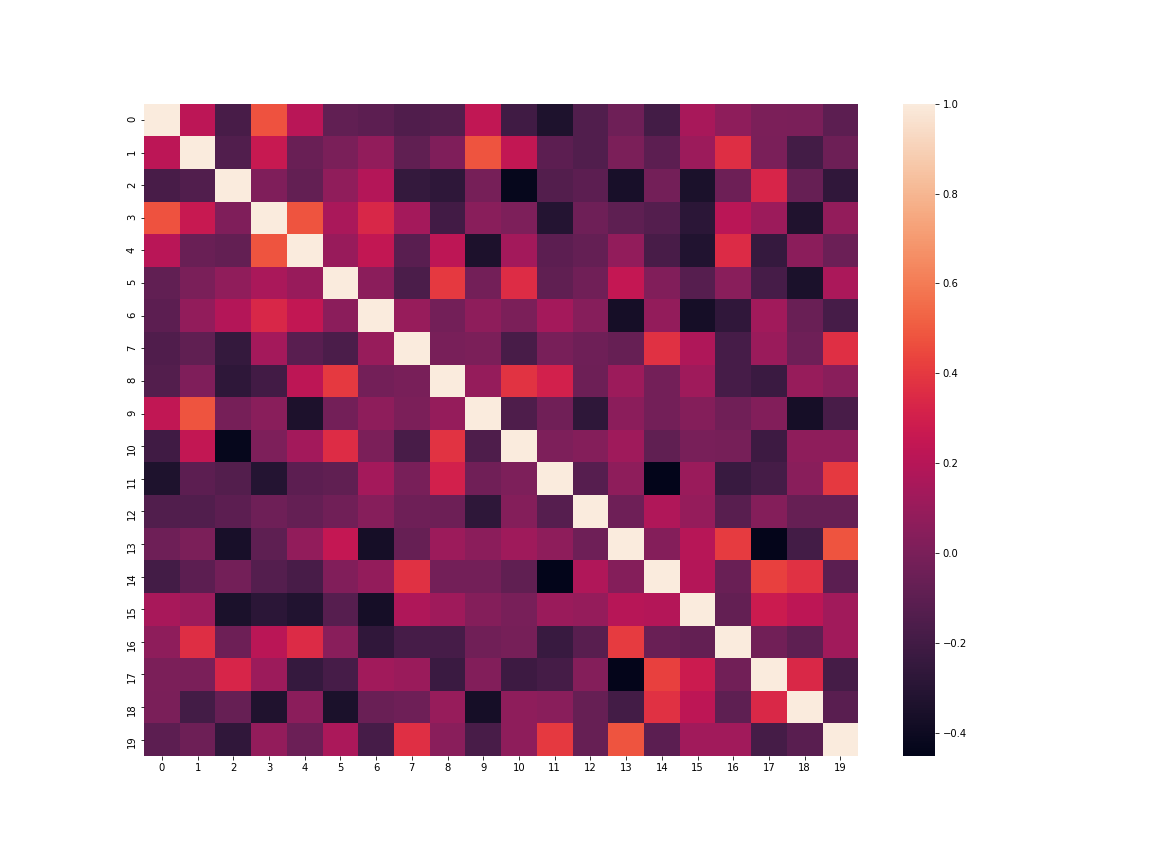
\includegraphics[width=0.7\linewidth]{figures/0106/hm_20t}
%\caption{}
%\label{fig:hm20t}
%\end{figure}
\subsection{Visualization}
To clearly demonstrate the representation for the word embedding space inside the parameters that obtained, we ran t-SNE algorithm to map the topic-word representation into 2-dimension continuous space. In figure \ref{fig:tsne20t25w2} and \ref{fig:tsne50t25w0}, demonstrate the t-SNE visualization of the topic-word distribution for 20Newsgroups for k=20 and k=50. 

We also compare the model with the ETM as displayed on figure \ref{fig:tsne20t50w1_etm}. In figure \ref{fig:tsne20t25w2}, the topic "space"(which consist of words like space, nasa, moon, etc) laying on the 2-dimensional space. The most neighboring topic includes "vehicles", "politics" and "america". For ETM, the nearest topic for "space" are "america", "operating system" and "vehicle". Generally, ETM do not able to distinct the words of topics into visible clusters, as shown on the figure, the upper part of word dots with different topic labels mix together. This implies ETM does not generate good enough topic-words representation to distinguish the difference between topics.
\begin{figure}
\centering
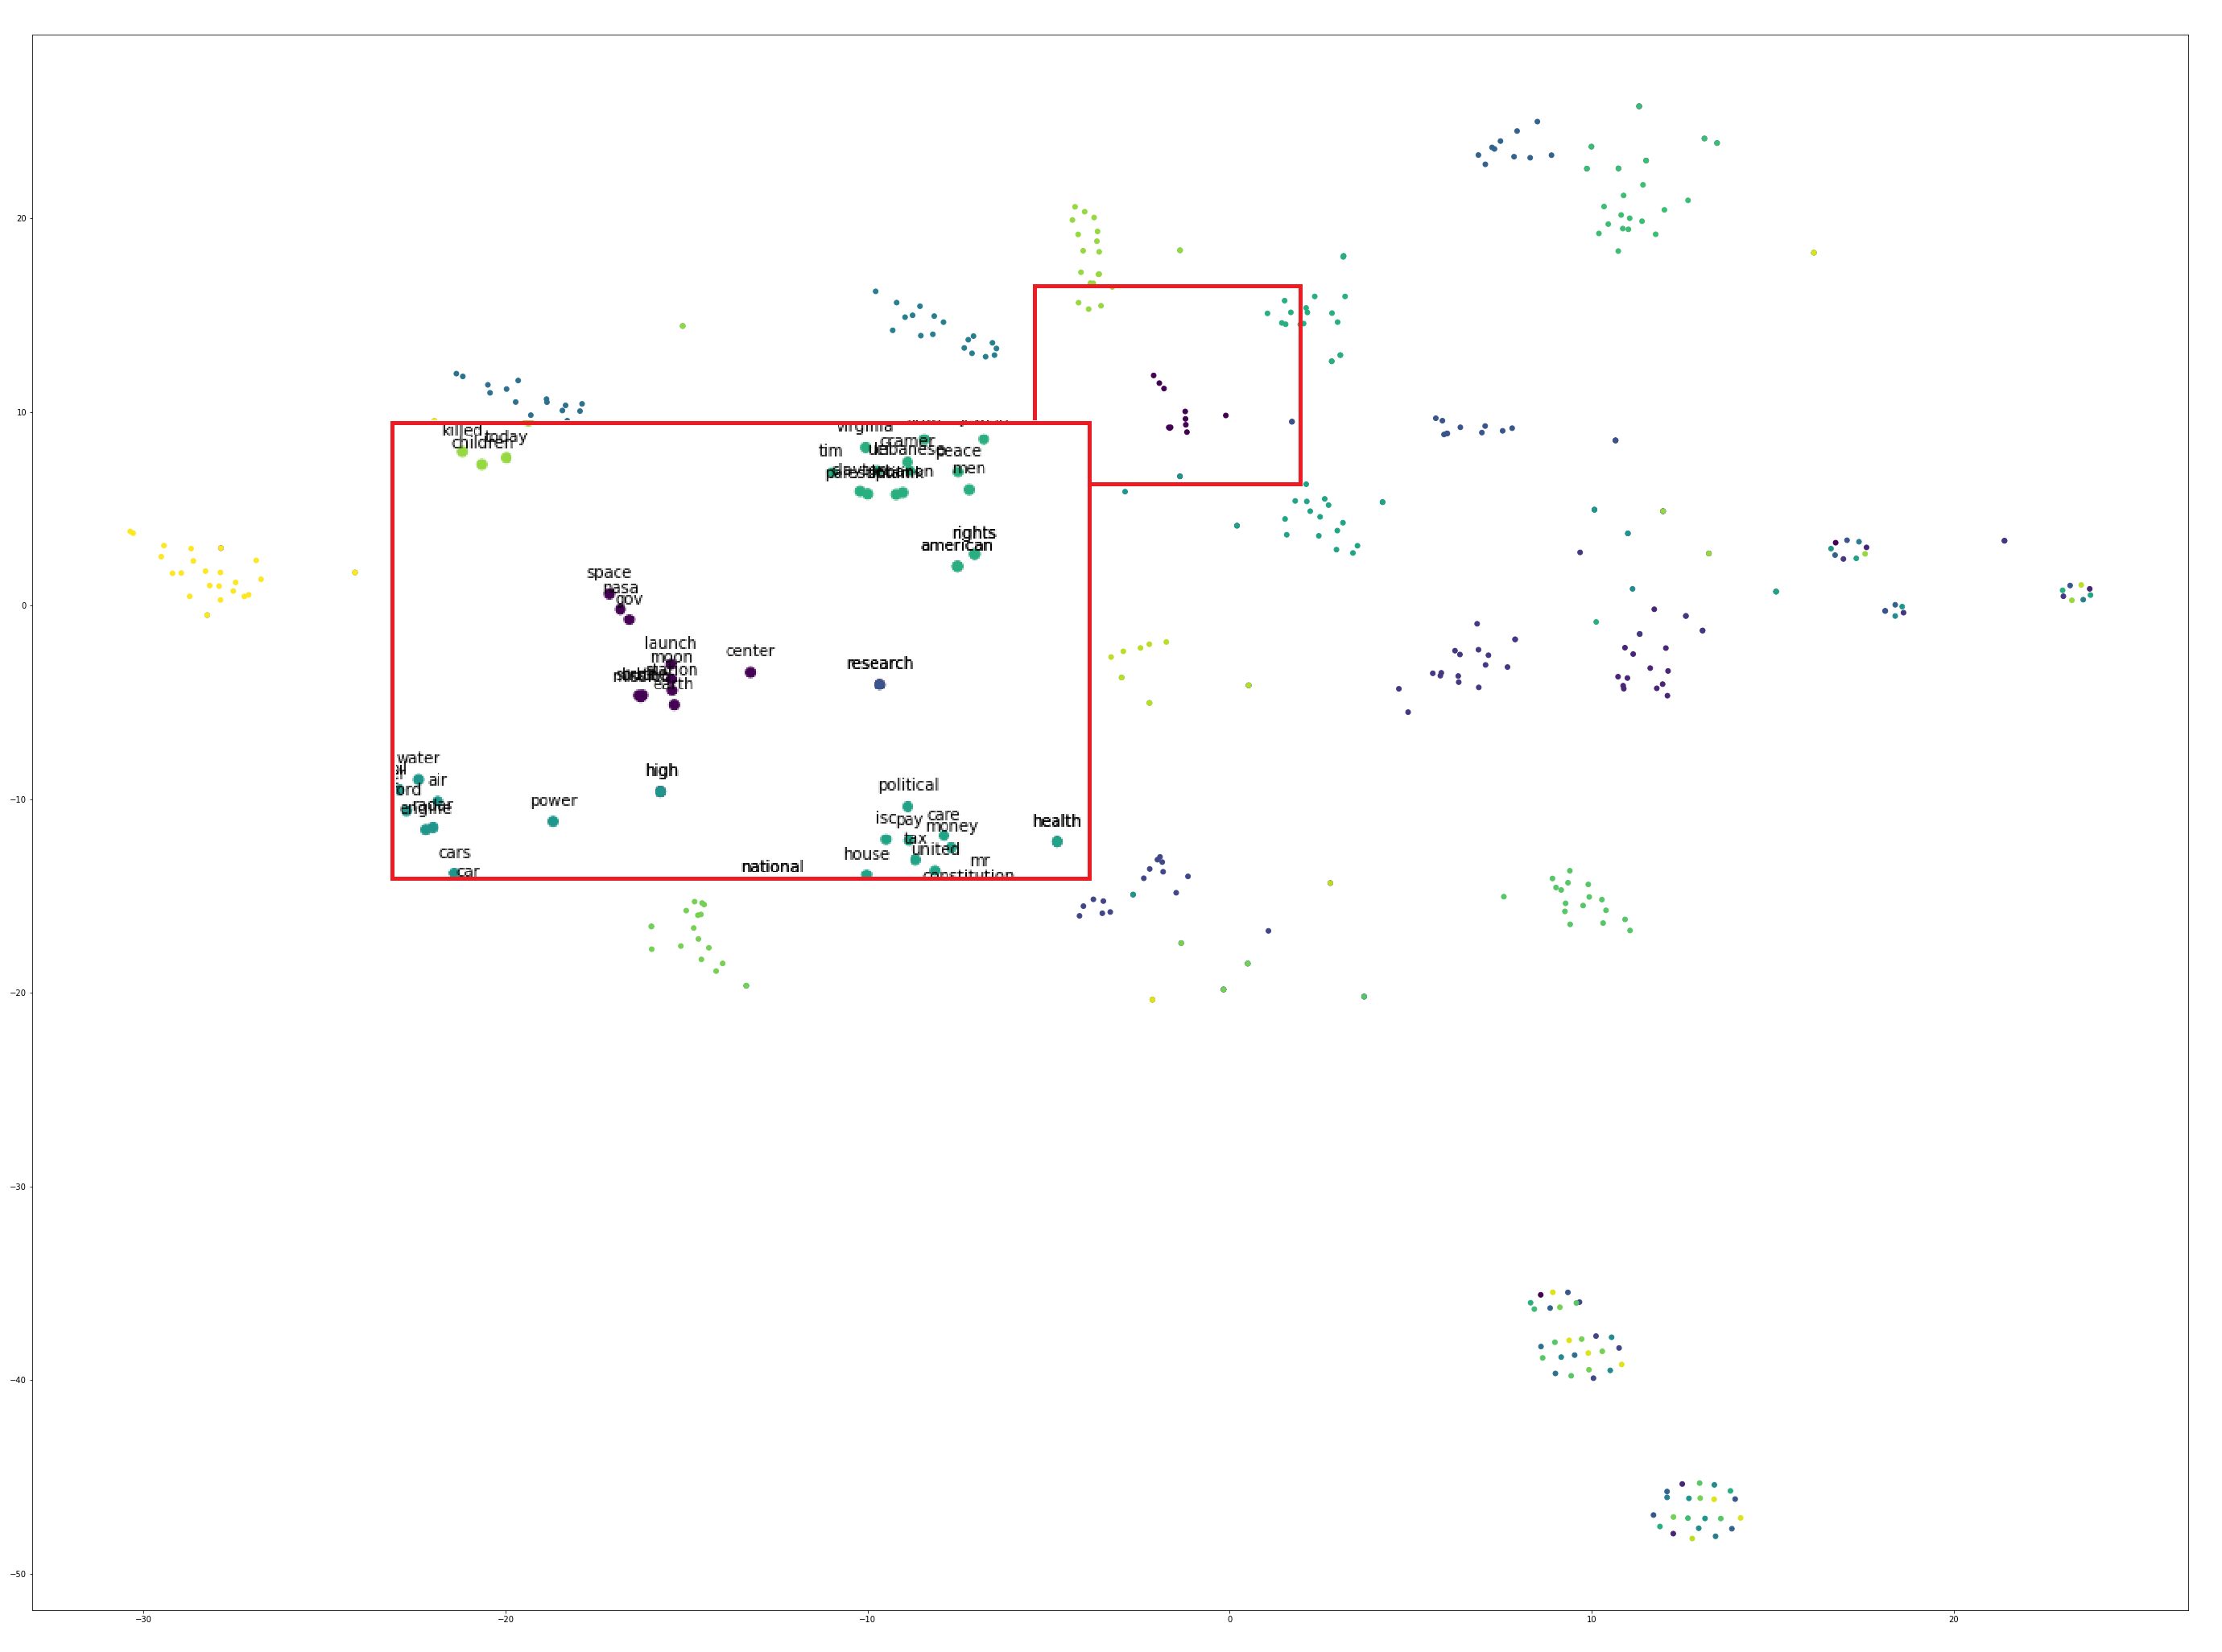
\includegraphics[width=1\linewidth]{figures/0908/tsne_20t_25w_2}
\caption{t-SNE Visualization for our model \#Topic:20}
\label{fig:tsne20t25w2}
\end{figure}
\begin{figure}
\centering
\includegraphics[width=1\linewidth]{"figures/0112/tsne_20t_50w(1) - Copy"}
\caption{t-SNE visualization for ETM \#Topic:20}
\label{fig:tsne20t50w1_etm}
\end{figure}
\begin{figure}
\centering
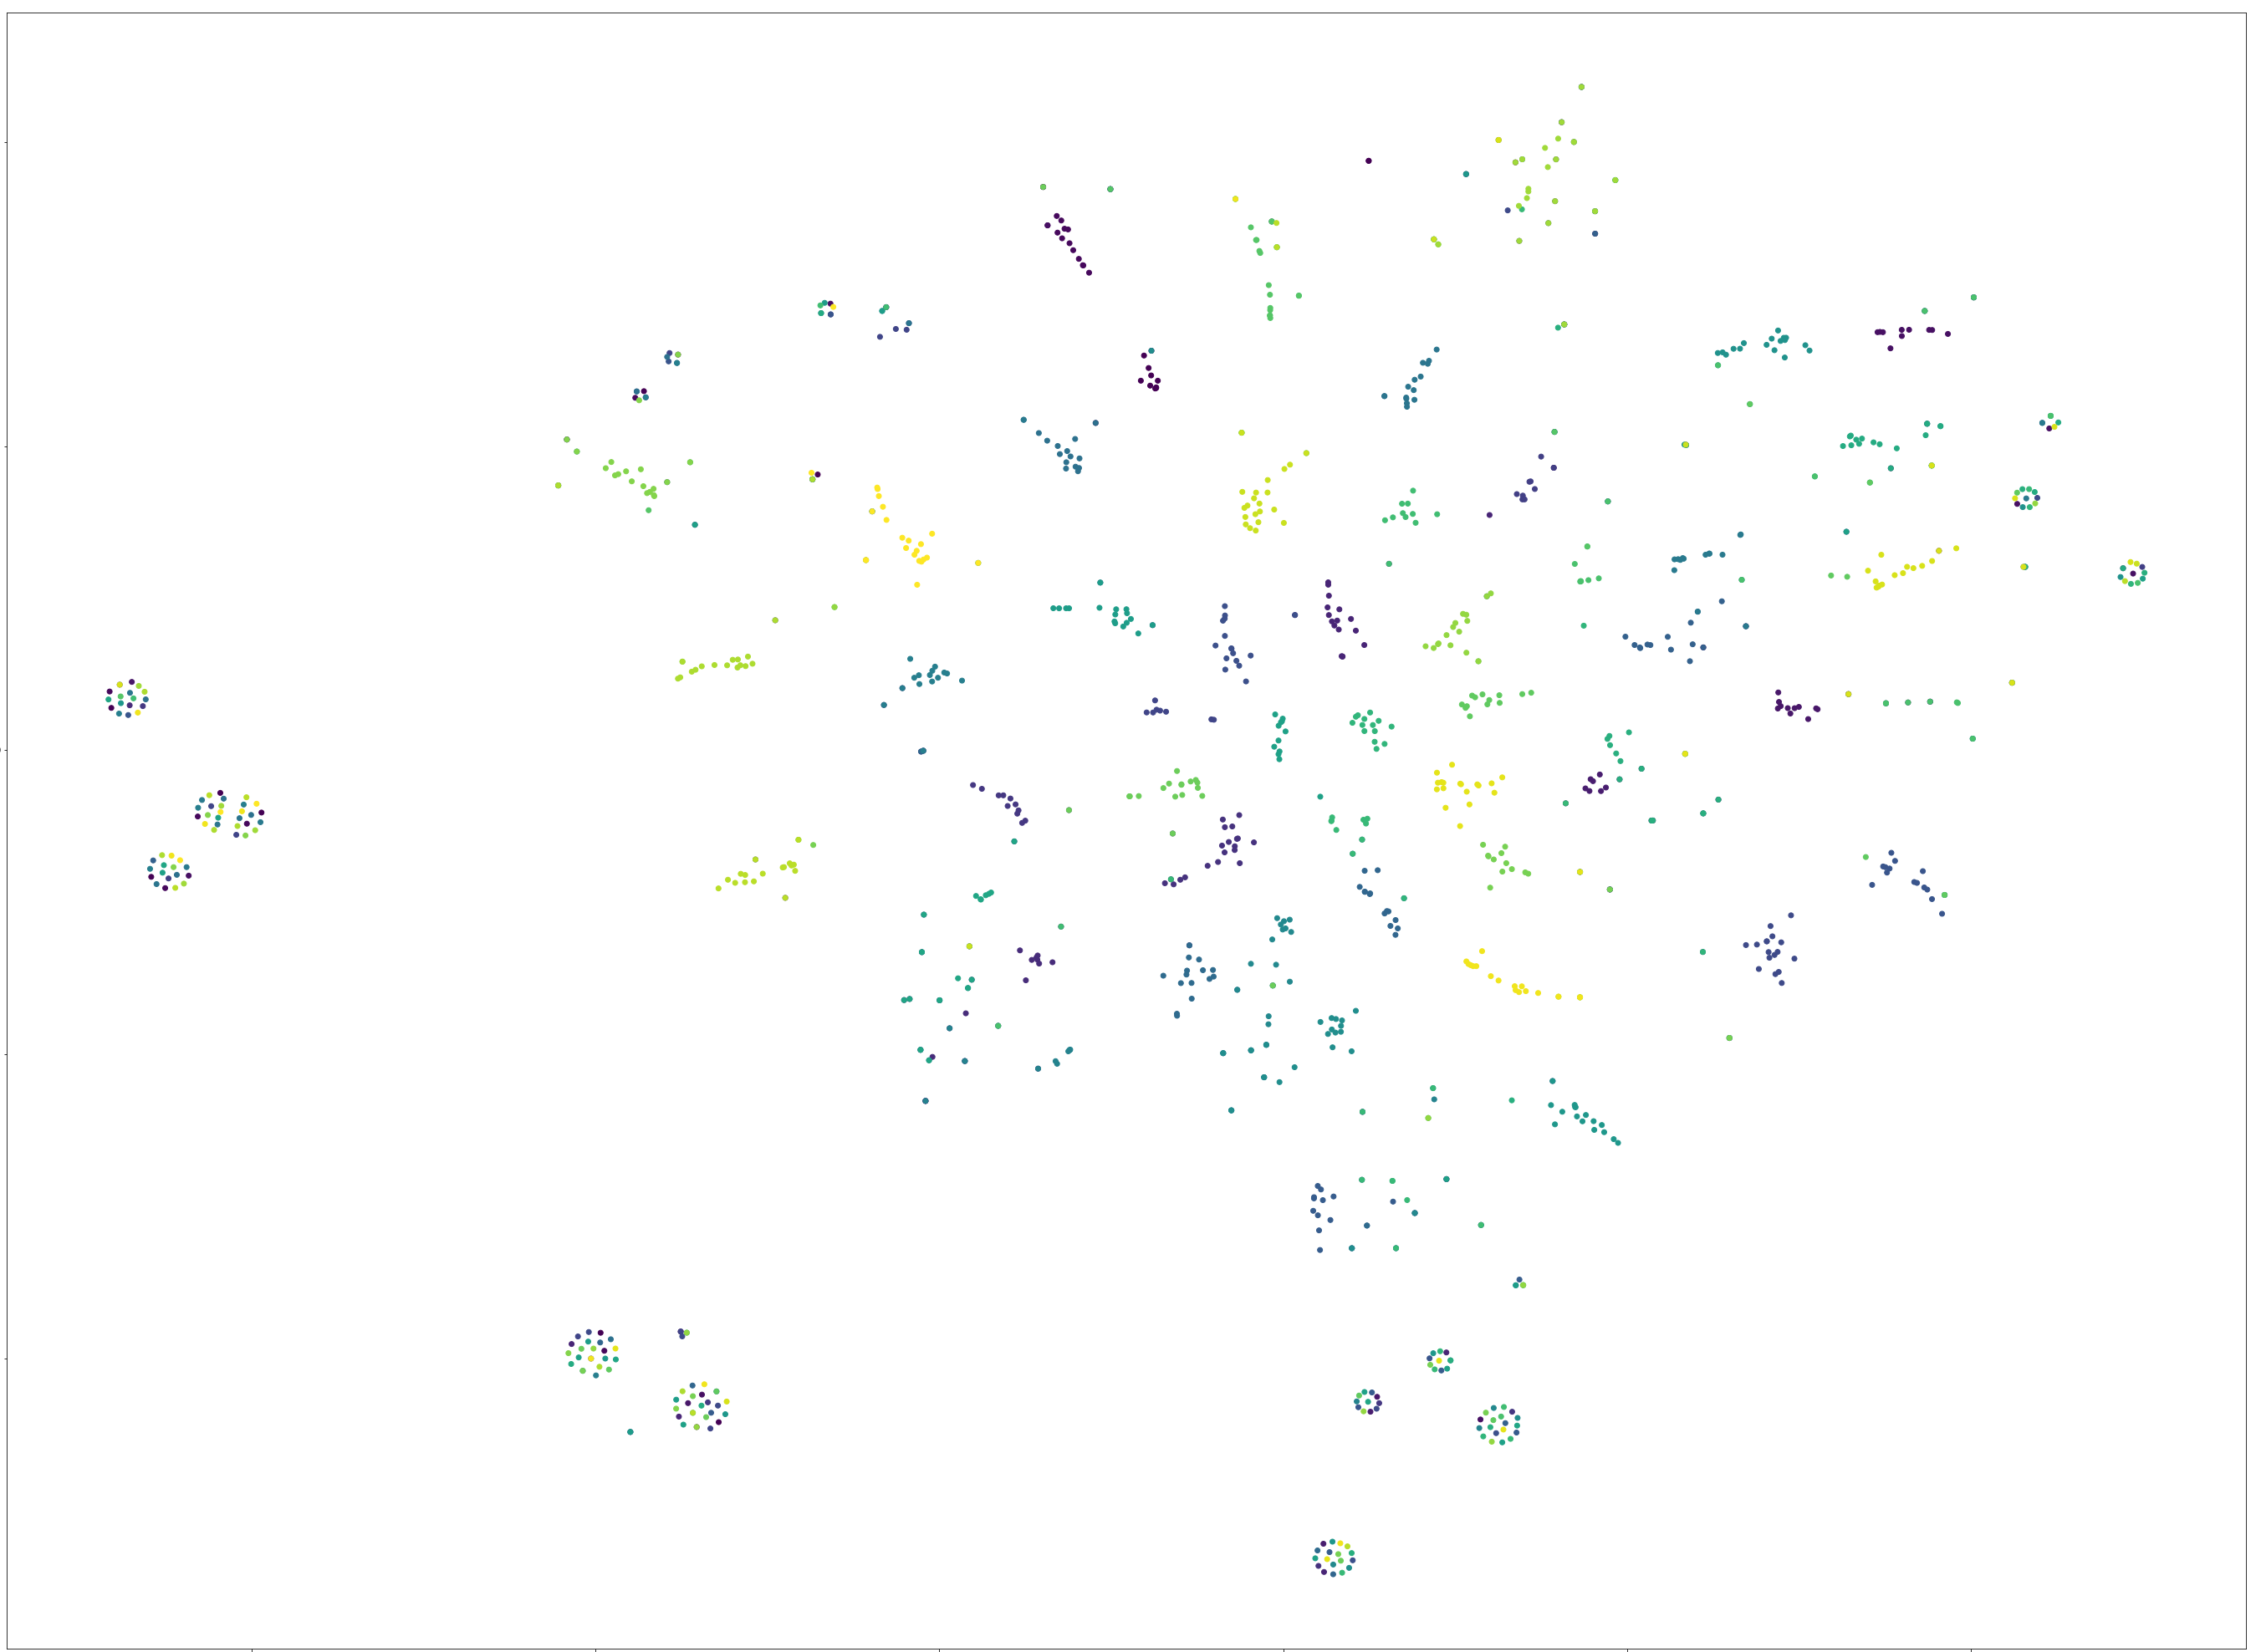
\includegraphics[width=1\linewidth]{figures/0908/tsne_50t_25w_0}
\caption{Visualization \#Topics:50}
\label{fig:tsne50t25w0}
\end{figure}
\subsection{Discussion}
We have compared our model with a number of state-of-the-art models on multiple data sets. 
% mention the perplexity is not a good measure
As we mentioned in previous section, perplexity may not be a good measure for comparing the topic models. Also, normally the perplexity for topic model are calculated using the posterior distribution, while the topic model using Autoencoding Variational Bayes(AEVB) are calculated using the variational lower bound\cite{srivastava_autoencoding_2017}. The results between these models may not able to draw conclusion easily. We have carefully compared the models on topic-model specific metrics like topic coherence and topic diversity. The result have
The result exhibits our model has a outstanding performance on obtaining high quality topic words over various of predefined topic numbers, especially in topic coherence score. In two of the metric we compared, topic coherence and topic diversity, our model shows its strength in generating high quality topics and diversified words. The comparison on the quantitative result also demonstrate that our model is robust to generate high quality topics upon the topic number defined increases.
% visualization
In the t-SNE visualization, our model also made a clearer representation on 2-dimensional space which implies a better intra-cluster divergence the model distinguish the difference between topics.